% Bloque para incorporar al póster conjunto.
% Requiere graphicx, booktabs y xcolor en el preámbulo principal.
\begin{minipage}[t]{0.48\linewidth}
\textbf{LectureKick}\par
\vspace{1mm}
\centering
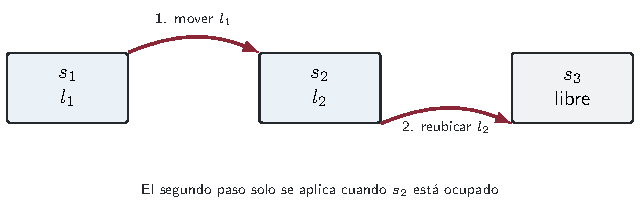
\includegraphics[width=\linewidth]{../figures/lecturekick.pdf}
\raggedright
\small
Una clase ocupa un nuevo hueco. Si ese destino estaba ocupado, la clase desplazada pasa a un tercer hueco libre. El operador amplía LectureMove y mantiene las restricciones duras.
\end{minipage}
\hfill
\begin{minipage}[t]{0.48\linewidth}
\textbf{Métodos y reproducción}\par
\vspace{1mm}
\small
\begin{tabular}{@{}p{0.31\linewidth}p{0.61\linewidth}@{}}
\toprule
Metaheurísticas & Exploran rápido, sensibles a parámetros \\
Híbridos & Reparación exacta y mejora local \\
Aprendizaje & Selección según la instancia \\
\bottomrule
\end{tabular}
\vspace{2mm}

\fbox{\parbox{0.92\linewidth}{\centering 19 instancias \quad 3 semillas\\192 s de referencia \quad 57 ejecuciones}}
\end{minipage}
